% How the trained CAE is split between the device and the computer (simplified).
% Top: training happens once, offline. Bottom: the live signal path.
\begin{tikzpicture}[
  font=\footnotesize,
  >={Stealth[length=1.8mm]},
  arr/.style={->, thick, black!70},
  dep/.style={->, thick, dashed, black!45},
  lbl/.style={font=\scriptsize, text=black!75, align=center},
  box/.style={draw=#1!80!black, fill=#1!12, line width=0.6pt, rounded corners=3pt,
              align=center, minimum height=1.5cm, text width=3.1cm},
  thumb/.style={inner sep=0pt}]

  \colorlet{encC}{blue!55!cyan}
  \colorlet{decC}{orange!85!red}
  \colorlet{latC}{green!50!black}
  \colorlet{offC}{black!60}

  % ---------------- live signal path ----------------
  \node[box=offC, text width=2.7cm] (ads) at (0,0) {\textbf{ADS1292R}\\[2pt]отвеждане II\\500 SPS, 24 bit};
  \node[box=encC] (esp) at (4.5,0) {\textbf{ESP32-S3}\\[2pt]ВЧ филтър\\прозорец 256\\\textbf{енкодер} \(\rightarrow z\)};
  \node[box=decC] (pc) at (10.0,0) {\textbf{Компютър}\\[2pt]\textbf{декодер}\\\(z \rightarrow \hat{x}\)};
  \node[thumb] (out) at (13.6,0) {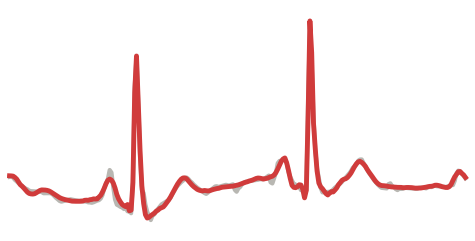
\includegraphics[width=2.2cm]{../figures/cae_out.png}};
  \node[lbl, below=1mm of out] {реконструиран ЕКГ};

  \node[font=\small, text=encC] at ($(esp.north east)+(-0.3,-0.3)$) {\faMicrochip};
  \node[font=\small, text=decC] at ($(pc.north east)+(-0.3,-0.3)$) {\faDesktop};

  \draw[arr] (ads) -- node[lbl, above] {SPI} (esp);
  \draw[->, thick, latC] (esp) -- node[lbl, above, text=latC!60!black] {32 B int8} node[lbl, below, text=latC!60!black] {на всеки 2.56 s} (pc);
  \draw[arr] (pc) -- (out);

  % ---------------- training, once ----------------
  \node[box=offC, fill=black!4, text width=4.2cm, minimum height=1.1cm] (train) at (7.15,2.9)
    {\textbf{Обучение на CAE} (веднъж, офлайн)\\PTB-XL, PyTorch, GPU};
  \draw[dep] (train.south) -- ++(0,-0.45) -| node[lbl, pos=0.75, left] {тегла на енкодера,\\филтър, мащаб, int8} (esp.north);
  \draw[dep] (train.south) -- ++(0,-0.45) -| node[lbl, pos=0.75, right] {тегла на\\декодера} (pc.north);
\end{tikzpicture}
